% !TEX root = thesis.tex
%%%%%%%%%%%%%%%%%%%%%%%%%%%%%%%%%%%%%%%%%%%%%%%%%%%%%%%%%%%%%%%%%%%%%%%%%%%%%%%%
\chapter{Разработка инструментальной среды}
%%%%%%%%%%%%%%%%%%%%%%%%%%%%%%%%%%%%%%%%%%%%%%%%%%%%%%%%%%%%%%%%%%%%%%%%%%%%%%%%

Разработка среды велась на языке Java 7 версии (OpenJDK Runtime Environment
(IcedTea 2.4.7)~\cite{Gosling2013}).

%%%%%%%%%%%%%%%%%%%%%%%%%%%%%%%%%%%%%%%%%%%%%%%%%%%%%%%%%%%%%%%%%%%%%%%%%%%%%%%%
\section{Структура проекта}
%%%%%%%%%%%%%%%%%%%%%%%%%%%%%%%%%%%%%%%%%%%%%%%%%%%%%%%%%%%%%%%%%%%%%%%%%%%%%%%%

В соответствии с архитектурой среды, приведенной в п.п.~\ref{sec:architecture},
проект разбит на 3 составляющих:

\begin{enumerate}
    \item Метамодель
    \item Преобразователи
    \item Инструментальная среда (графический интерфейс, процедуры визуализации
    и анализа)
\end{enumerate}

\nomenclature{POM}{Project Object Model, способ описания проекта в система
автоматизированной сборки Maven}

Сборка проекта производится при помощи фреймворка для автоматизации сборки
Apache Maven. Данный фреймворк позволяет декларативным образом описывать процесс
сборки проекта, фокусируясь на его структуре, используя различные плагины для
организации фаз построения~\cite{Maven2001-2005}. Вся информация содержится в
XML-файле под названием pom.xml (Project Object Model). Одной из отличительной
особенностей Maven является наличие центрального репозитория, что сильно
упрощает управление зависимостями разрабатываемого проекта. Добавляя необходимые
библиотеки в pom.xml, они будут автоматически скачены из центрального
репозитория и размещены в локальном репозитории для дальнейшего использования в
цикле сборки проекта.

Проект разделен на три maven-модуля, связь между которыми изображена на
рис.~\ref{fig:project_structure}.

\begin{figure}[ht]
    \begin{center}
        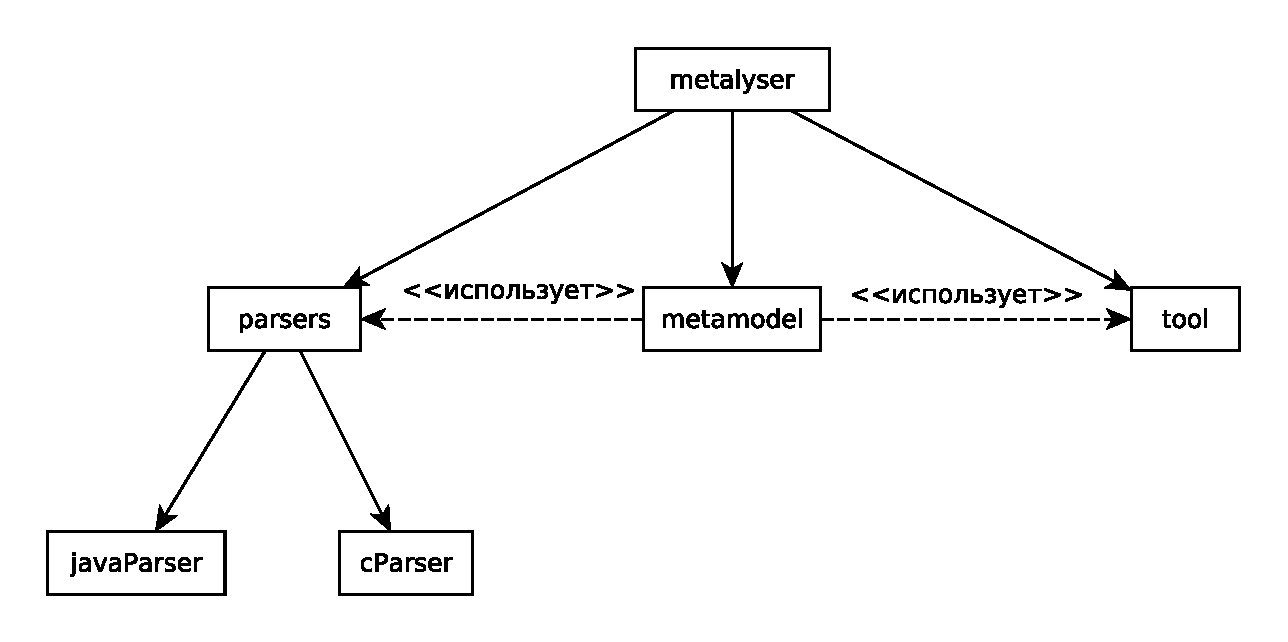
\includegraphics[width=\textwidth]{project_structure.eps}
    \end{center}
    \caption{Структура maven-проекта}
    \label{fig:project_structure}
\end{figure}

Рассмотрим подробнее приведенную структуру:

\begin{enumerate}
    \item Модуль верхнего уровня называется \texttt{metalyser} (Meta-Analyser) и
    является корнем всего проекта. В нем размещаются зависимости и плагины maven,
    необходимые для сборки всей программной системы.
    \item Модуль \texttt{parsers} является родительским модулем для
    преобразователей языка Java и C, поставляемых вместе с разработанной средой.
    \item Модуль \texttt{javaParser} является преобразователем для языка Java.
    Аналогично, модуль \texttt{cParser} используется для импортирования систем,
    написанных на языке C.
    \item Модуль \texttt{metamodel} является реализацией метамодели,
    описывающей анализируемую систему. Данный модуль реализован в виде
    библиотеки классов и не предназначен для непосредственного использования
    (он не содержит Main-класса для запуска), а используется в виде зависимости
    в остальных модулях системы.
    \item Модуль \texttt{tool} является реализацией инструментальной среды.
\end{enumerate}

%%%%%%%%%%%%%%%%%%%%%%%%%%%%%%%%%%%%%%%%%%%%%%%%%%%%%%%%%%%%%%%%%%%%%%%%%%%%%%%%
\section{Разработка метамодели}
%%%%%%%%%%%%%%%%%%%%%%%%%%%%%%%%%%%%%%%%%%%%%%%%%%%%%%%%%%%%%%%%%%%%%%%%%%%%%%%%

На основе анализа возможной архитектуры метамодели (см.
п.п.~\ref{sec:metamodel_architecture}), было принято взять за основу
архитектуру, предложенную стандартом MOF. Недостатком данной архитектуры
является ее громоздкость: полученные метамодели охватывают широкий спектр
возможных задач, что делает их достаточно объемными и сложными в использовании.
Исходя из требований к системе, было решено модифицировать исходную архитектуру,
а именно были убраны отдельные классы для отображения отношений между объектами.
Вместо этого ссылки на зависимые объекты хранятся непосредственно в самих
классах. Из-за этого теряется семантическая информация о видах отношений, но
намного сокращается количество используемых классов, что сильно упрощает
использование библиотеки.

Таким образом, полученная метамодель не является полностью MOF-совместимой, но,
если в дальнейшем развитии проекта будет необходима такая совместимость для
взаимодействия со сторонними приложениями, не составит труда привести ее к
полной совместимости.

Принимая во внимание все перечисленные замечания, была разработана
соответствующая структура метамодели. Краткая UML-диаграмма классов приведена на
рис.~\ref{fig:metamodel_uml}. Стоит отметить, что на данной диаграмме, для
уменьшения ее размеров, были опущены все методы, отношения между классами и
некоторые наследники основных суперклассов.

\newpage
\begin{sidewaysfigure}[ht!]
    \begin{center}
        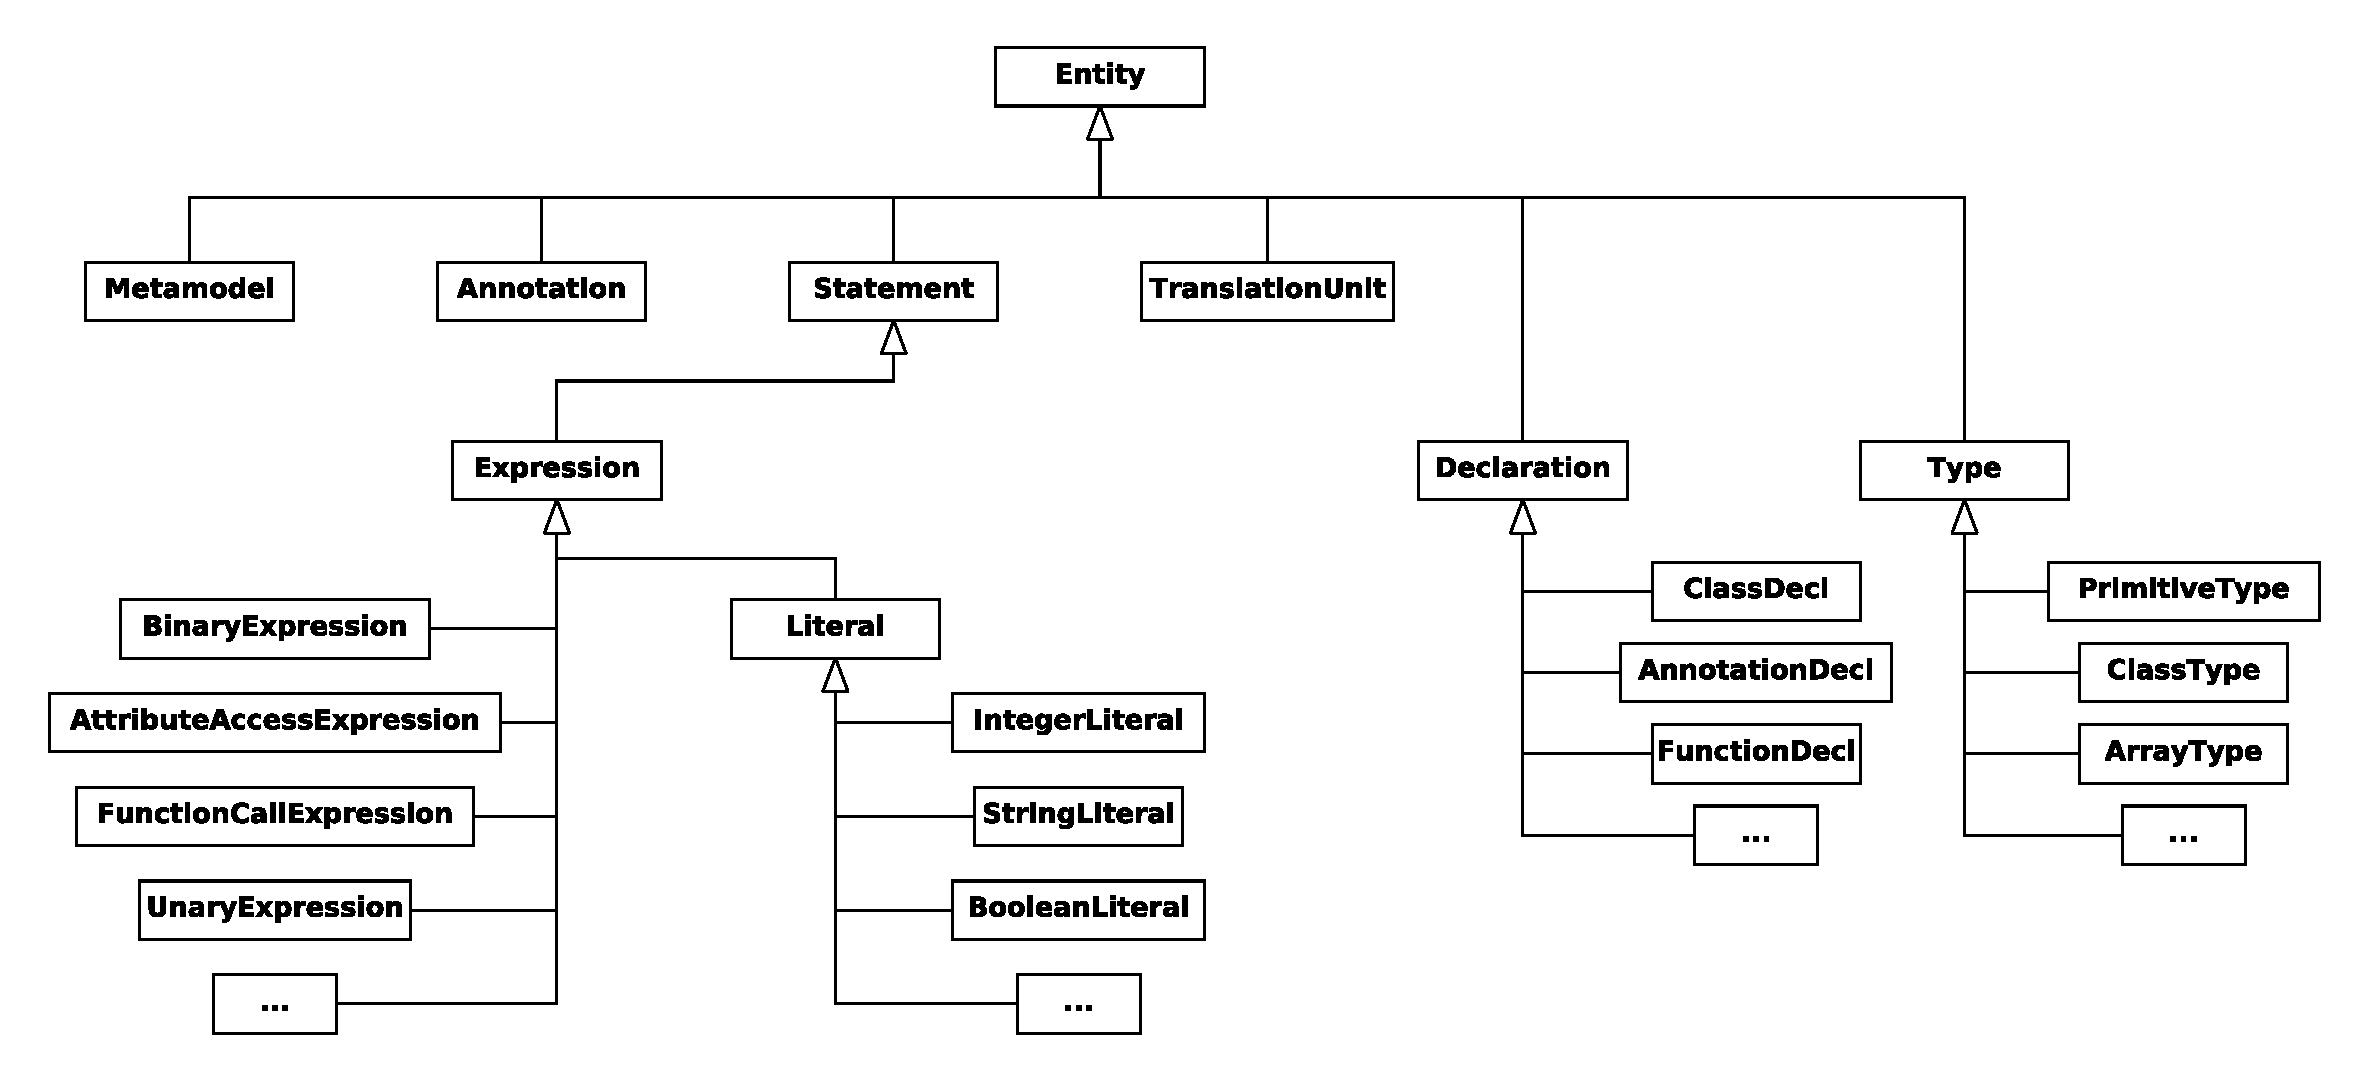
\includegraphics[width=\textwidth]{metamodel_uml.eps}
    \end{center}
    \caption{Упрощенная диаграмма классов метамодели}
    \label{fig:metamodel_uml}
\end{sidewaysfigure}

Рассмотрим подробнее некоторые из классов:

\subsubsection{Entity}

\begin{lstlisting}
public interface Entity {
    public void accept(final Visitor visitor);
}
\end{lstlisting}

От интерфейса \texttt{Entity} наследуются все классы метамодели. Класс содержит
лишь один метод - \texttt{accept}, который необходим для обхода дерева, которое
представляет из себя построенная модель. Таким образом для проведения анализа
метамодели был реализован паттерн "Посетитель" (подробнее про обход
дерева объектов описано в п.п. \todo{вставить номер подпункта}).

\subsubsection{Metamodel}

\begin{lstlisting}
public class Metamodel implements Entity {
    private final List<TranslationUnit> units;

    ...
}
\end{lstlisting}

Данный класс является контейнером верхнего уровня для объектов типа
\texttt{TranslationUnit}. Он предназначен для сборки результатов работы
преобразователей над каждым из файлов с исходным кодом анализируемой программной
системы.

\subsubsection{TranslationUnit}

\begin{lstlisting}
public class TranslationUnit implements Entity {
    private final List<Import> imports;
    private final List<Declaration> types;

    ...
}
\end{lstlisting}

Класс \texttt{TranslationUnit} отображает одну единицу трансляции при работе
преобразователя. Обычно ей соответствует один файл с исходным кодом (за
исключением, например, языка C, где в каждый файл на этапе работы препроцессора
вставляется текст используемых заголовочных или любых других файлов,
подключенных при помощи директивы \texttt{\#include}). Таким образом, обычно при
трансляции всей анализируемой системы в результате работы преобразователя
будет получено несколько объектов типа \texttt{TranslationUnit}, которые затем
должны быть объединены в один объект типа \texttt{Metamodel}.
